\documentclass[UTF8]{ctexbeamer}
\usefonttheme[onlymath]{serif}
\usepackage{listings}  
\usepackage{fontspec}  
\setmonofont{Consolas}  
\usepackage{graphicx}
\usepackage{amsmath}
\usetheme{metropolis}           % Use metropolis theme
\title{OFDM频域模型验证}
\date{\today}
\author{李昊}
\institute{通信系统仿真大作业}
\begin{document}
  \maketitle
  \section{整体框架}
  \begin{frame}{整体框架--流程描述}
	\begin{figure}
	  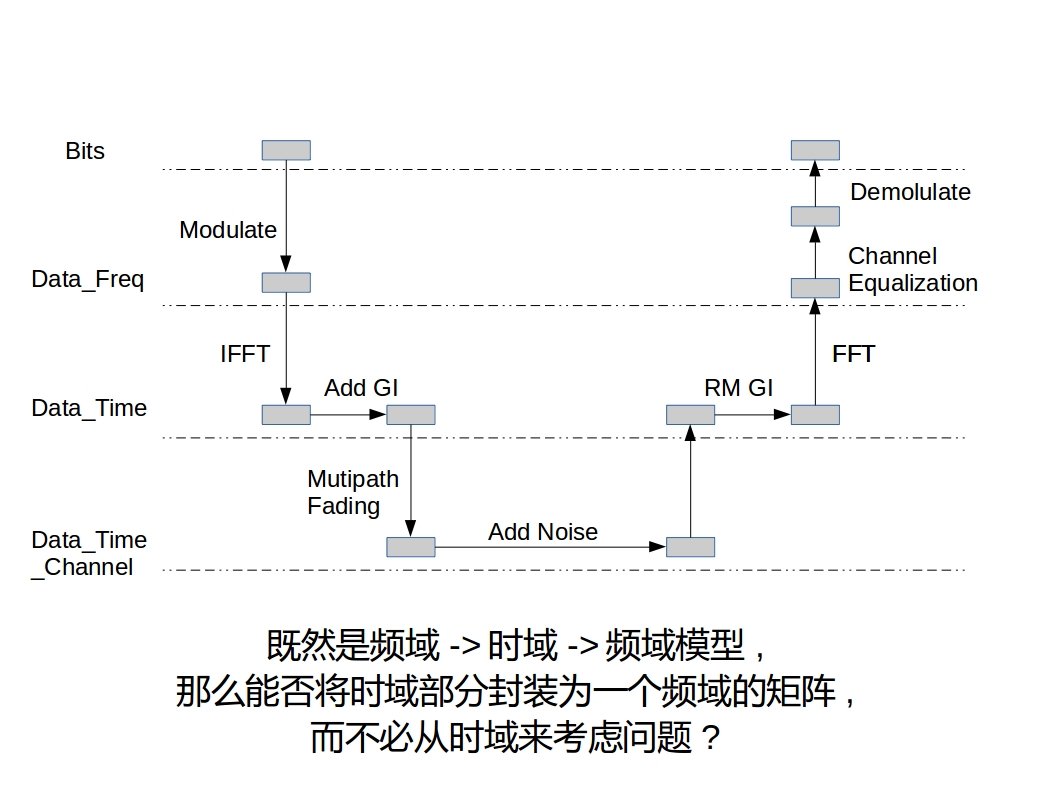
\includegraphics[width=\textwidth]{figure/top.jpg}
	\end{figure}
  \end{frame}
  \begin{frame}{整体框架--数学描述}
	\begin{equation*}
	  \begin{aligned}
	\hat Y &= FHF^{-1}X+FW \\
	 Y &= \hat Y * \frac{H_0^*}{||H_0||^2}\\
	 H_0 &= \frac{P_{Re}}{P_{Tr}} \\
	  \end{aligned}
	\end{equation*}
  \end{frame}

  \section{数字实现}
  \begin{frame}{数字实现---信道矩阵}
	\\方法一:加循环前缀和循环延时
	\scalebox{0.5}{ 	\begin{equation*}
	  \begin{aligned}
		HX &= \\ &
		\begin{pmatrix}
		 h(Q-1)&\ldots  &h(0)  & \ldots  & 0 & 0 & 0  & \ldots & 0 \\ 
		 0&h(Q-1)&\ldots  &h(0)  & \ldots  & 0 & 0 & 0  & \ldots  \\ 
		 \ldots&0&h(Q-1)&\ldots  &h(0)  & \ldots  & 0 & 0 & 0    \\ 
		0& \ldots&0&h(Q-1)&\ldots  &h(0)  & \ldots  & 0 & 0     \\ 
		0&0& \ldots&0&h(Q-1)&\ldots  &h(0)  & \ldots  & 0      \\ 
		0&0&0& \ldots&0&h(Q-1)&\ldots  &h(0)  & \ldots        \\ 
		\ldots&0&0&0& \ldots&0&h(Q-1)&\ldots  &h(0)   \\ 
		 \end{pmatrix}
		\times 
		\begin{pmatrix}
		X(-N_{CP}-Q+1)\\ 
		\ldots\\ 
		X(-N_{CP})\\ 
		\ldots\\ 
		  X(-1)\\ 
		  X(0)\\ 
		  X(1)\\
		\ldots\\
		  X(N-1)\\
		\end{pmatrix}
		\\&
	if \; $n<0$, then \; X(n)=X(n+N)
	  \end{aligned}
	\end{equation*}

 }
	\\方法二:由于循环矩阵的特性, 在矩阵运算中可以将其省略
	\scalebox{0.5}{ \begin{equation*}
  \begin{aligned}
	HX&=\\ &
\begin{pmatrix}
h(0) & 0 & \ldots & h(Q-1) & \ldots & h(1)\\ 
h(1)&h(0) & 0 & \ldots & h(Q-1) & \ldots \\ 
\ldots &h(1)&h(0) & 0 & \ldots & h(Q-1) \\ 
h(Q-1)&\ldots &h(1)&h(0) & 0 & \ldots  \\ 
\ldots&h(Q-1)&\ldots &h(1)&h(0) & 0  \\ 
0&\ldots&h(Q-1)&\ldots &h(1)&h(0)   \\ 
\end{pmatrix}
\times 
\begin{pmatrix}
X(0)\\ 
X(1)\\
\ldots\\
\ldots\\
\ldots\\
\ldots\\
X(N-1)\\

\end{pmatrix}
  \end{aligned}
\end{equation*}
 }
  \end{frame}
  \begin{frame}{数字实现--- $F, F^{-1}, W$ }
	\input{math/FW}
  \end{frame}
  \begin{frame}{数字实现--- 主函数 }
	\documentclass[UTF8]{ctexbeamer}
\usefonttheme[onlymath]{serif}
\usepackage{listings}  
\usepackage{fontspec}  
\setmonofont{Consolas}  
\usepackage{graphicx}
\usepackage{amsmath}
\usetheme{metropolis}           % Use metropolis theme
\title{OFDM频域模型验证}
\date{\today}
\author{李昊}
\institute{通信系统仿真大作业}
\begin{document}
  \maketitle
  \section{整体框架}
  \begin{frame}{整体框架--流程描述}
	\begin{figure}
	  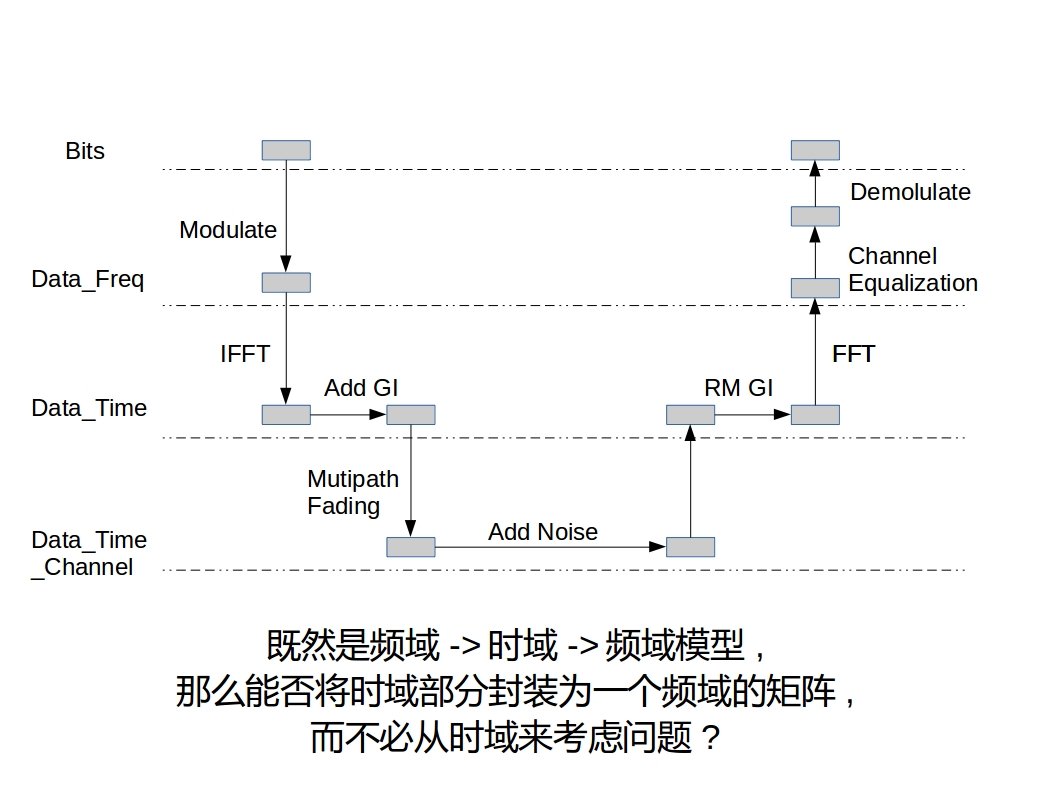
\includegraphics[width=\textwidth]{figure/top.jpg}
	\end{figure}
  \end{frame}
  \begin{frame}{整体框架--数学描述}
	\begin{equation*}
	  \begin{aligned}
	\hat Y &= FHF^{-1}X+FW \\
	 Y &= \hat Y * \frac{H_0^*}{||H_0||^2}\\
	 H_0 &= \frac{P_{Re}}{P_{Tr}} \\
	  \end{aligned}
	\end{equation*}
  \end{frame}

  \section{数字实现}
  \begin{frame}{数字实现---信道矩阵}
	\\方法一:加循环前缀和循环延时
	\scalebox{0.5}{ 	\begin{equation*}
	  \begin{aligned}
		HX &= \\ &
		\begin{pmatrix}
		 h(Q-1)&\ldots  &h(0)  & \ldots  & 0 & 0 & 0  & \ldots & 0 \\ 
		 0&h(Q-1)&\ldots  &h(0)  & \ldots  & 0 & 0 & 0  & \ldots  \\ 
		 \ldots&0&h(Q-1)&\ldots  &h(0)  & \ldots  & 0 & 0 & 0    \\ 
		0& \ldots&0&h(Q-1)&\ldots  &h(0)  & \ldots  & 0 & 0     \\ 
		0&0& \ldots&0&h(Q-1)&\ldots  &h(0)  & \ldots  & 0      \\ 
		0&0&0& \ldots&0&h(Q-1)&\ldots  &h(0)  & \ldots        \\ 
		\ldots&0&0&0& \ldots&0&h(Q-1)&\ldots  &h(0)   \\ 
		 \end{pmatrix}
		\times 
		\begin{pmatrix}
		X(-N_{CP}-Q+1)\\ 
		\ldots\\ 
		X(-N_{CP})\\ 
		\ldots\\ 
		  X(-1)\\ 
		  X(0)\\ 
		  X(1)\\
		\ldots\\
		  X(N-1)\\
		\end{pmatrix}
		\\&
	if \; $n<0$, then \; X(n)=X(n+N)
	  \end{aligned}
	\end{equation*}

 }
	\\方法二:由于循环矩阵的特性, 在矩阵运算中可以将其省略
	\scalebox{0.5}{ \begin{equation*}
  \begin{aligned}
	HX&=\\ &
\begin{pmatrix}
h(0) & 0 & \ldots & h(Q-1) & \ldots & h(1)\\ 
h(1)&h(0) & 0 & \ldots & h(Q-1) & \ldots \\ 
\ldots &h(1)&h(0) & 0 & \ldots & h(Q-1) \\ 
h(Q-1)&\ldots &h(1)&h(0) & 0 & \ldots  \\ 
\ldots&h(Q-1)&\ldots &h(1)&h(0) & 0  \\ 
0&\ldots&h(Q-1)&\ldots &h(1)&h(0)   \\ 
\end{pmatrix}
\times 
\begin{pmatrix}
X(0)\\ 
X(1)\\
\ldots\\
\ldots\\
\ldots\\
\ldots\\
X(N-1)\\

\end{pmatrix}
  \end{aligned}
\end{equation*}
 }
  \end{frame}
  \begin{frame}{数字实现--- $F, F^{-1}, W$ }
	\input{math/FW}
  \end{frame}
  \begin{frame}{数字实现--- 主函数 }
	\documentclass[UTF8]{ctexbeamer}
\usefonttheme[onlymath]{serif}
\usepackage{listings}  
\usepackage{fontspec}  
\setmonofont{Consolas}  
\usepackage{graphicx}
\usepackage{amsmath}
\usetheme{metropolis}           % Use metropolis theme
\title{OFDM频域模型验证}
\date{\today}
\author{李昊}
\institute{通信系统仿真大作业}
\begin{document}
  \maketitle
  \section{整体框架}
  \begin{frame}{整体框架--流程描述}
	\begin{figure}
	  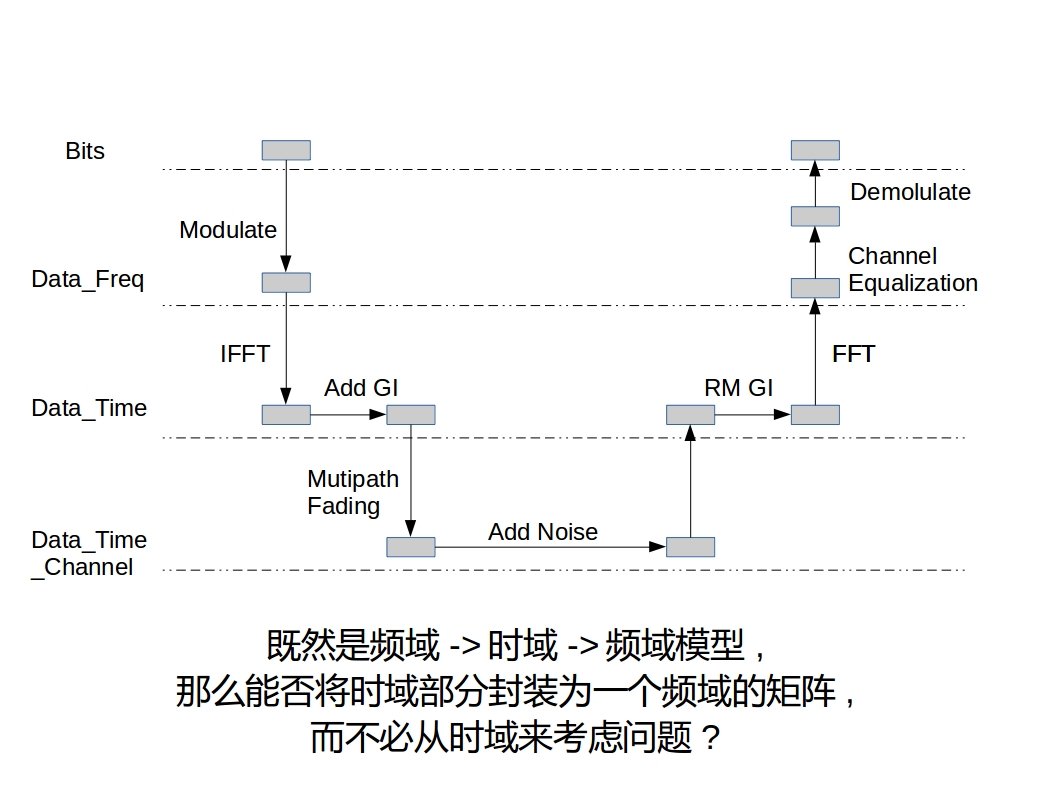
\includegraphics[width=\textwidth]{figure/top.jpg}
	\end{figure}
  \end{frame}
  \begin{frame}{整体框架--数学描述}
	\begin{equation*}
	  \begin{aligned}
	\hat Y &= FHF^{-1}X+FW \\
	 Y &= \hat Y * \frac{H_0^*}{||H_0||^2}\\
	 H_0 &= \frac{P_{Re}}{P_{Tr}} \\
	  \end{aligned}
	\end{equation*}
  \end{frame}

  \section{数字实现}
  \begin{frame}{数字实现---信道矩阵}
	\\方法一:加循环前缀和循环延时
	\scalebox{0.5}{ 	\begin{equation*}
	  \begin{aligned}
		HX &= \\ &
		\begin{pmatrix}
		 h(Q-1)&\ldots  &h(0)  & \ldots  & 0 & 0 & 0  & \ldots & 0 \\ 
		 0&h(Q-1)&\ldots  &h(0)  & \ldots  & 0 & 0 & 0  & \ldots  \\ 
		 \ldots&0&h(Q-1)&\ldots  &h(0)  & \ldots  & 0 & 0 & 0    \\ 
		0& \ldots&0&h(Q-1)&\ldots  &h(0)  & \ldots  & 0 & 0     \\ 
		0&0& \ldots&0&h(Q-1)&\ldots  &h(0)  & \ldots  & 0      \\ 
		0&0&0& \ldots&0&h(Q-1)&\ldots  &h(0)  & \ldots        \\ 
		\ldots&0&0&0& \ldots&0&h(Q-1)&\ldots  &h(0)   \\ 
		 \end{pmatrix}
		\times 
		\begin{pmatrix}
		X(-N_{CP}-Q+1)\\ 
		\ldots\\ 
		X(-N_{CP})\\ 
		\ldots\\ 
		  X(-1)\\ 
		  X(0)\\ 
		  X(1)\\
		\ldots\\
		  X(N-1)\\
		\end{pmatrix}
		\\&
	if \; $n<0$, then \; X(n)=X(n+N)
	  \end{aligned}
	\end{equation*}

 }
	\\方法二:由于循环矩阵的特性, 在矩阵运算中可以将其省略
	\scalebox{0.5}{ \begin{equation*}
  \begin{aligned}
	HX&=\\ &
\begin{pmatrix}
h(0) & 0 & \ldots & h(Q-1) & \ldots & h(1)\\ 
h(1)&h(0) & 0 & \ldots & h(Q-1) & \ldots \\ 
\ldots &h(1)&h(0) & 0 & \ldots & h(Q-1) \\ 
h(Q-1)&\ldots &h(1)&h(0) & 0 & \ldots  \\ 
\ldots&h(Q-1)&\ldots &h(1)&h(0) & 0  \\ 
0&\ldots&h(Q-1)&\ldots &h(1)&h(0)   \\ 
\end{pmatrix}
\times 
\begin{pmatrix}
X(0)\\ 
X(1)\\
\ldots\\
\ldots\\
\ldots\\
\ldots\\
X(N-1)\\

\end{pmatrix}
  \end{aligned}
\end{equation*}
 }
  \end{frame}
  \begin{frame}{数字实现--- $F, F^{-1}, W$ }
	\input{math/FW}
  \end{frame}
  \begin{frame}{数字实现--- 主函数 }
	\documentclass[UTF8]{ctexbeamer}
\usefonttheme[onlymath]{serif}
\usepackage{listings}  
\usepackage{fontspec}  
\setmonofont{Consolas}  
\usepackage{graphicx}
\usepackage{amsmath}
\usetheme{metropolis}           % Use metropolis theme
\title{OFDM频域模型验证}
\date{\today}
\author{李昊}
\institute{通信系统仿真大作业}
\begin{document}
  \maketitle
  \section{整体框架}
  \begin{frame}{整体框架--流程描述}
	\begin{figure}
	  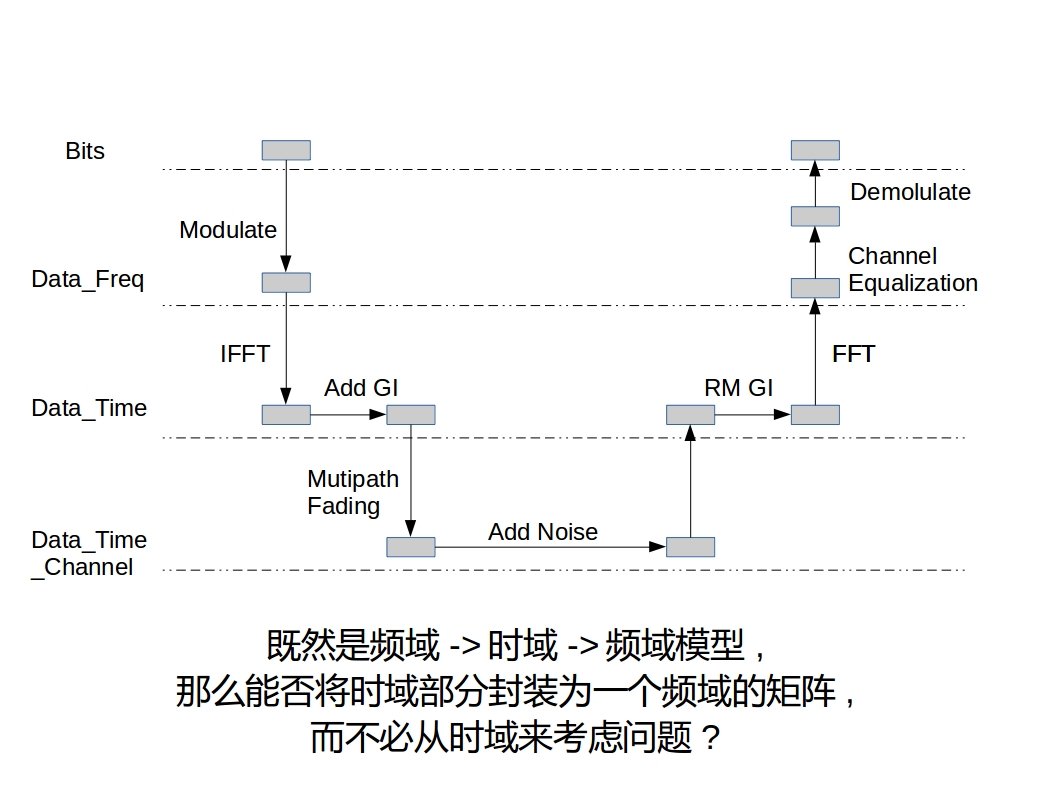
\includegraphics[width=\textwidth]{figure/top.jpg}
	\end{figure}
  \end{frame}
  \begin{frame}{整体框架--数学描述}
	\begin{equation*}
	  \begin{aligned}
	\hat Y &= FHF^{-1}X+FW \\
	 Y &= \hat Y * \frac{H_0^*}{||H_0||^2}\\
	 H_0 &= \frac{P_{Re}}{P_{Tr}} \\
	  \end{aligned}
	\end{equation*}
  \end{frame}

  \section{数字实现}
  \begin{frame}{数字实现---信道矩阵}
	\\方法一:加循环前缀和循环延时
	\scalebox{0.5}{ \input{math/H_old} }
	\\方法二:由于循环矩阵的特性, 在矩阵运算中可以将其省略
	\scalebox{0.5}{ \input{math/H_new} }
  \end{frame}
  \begin{frame}{数字实现--- $F, F^{-1}, W$ }
	\input{math/FW}
  \end{frame}
  \begin{frame}{数字实现--- 主函数 }
	\input{code/main}
  \end{frame}
  \begin{frame}{数字实现--- 方法二 }
	\input{code/way_matrix}
  \end{frame}
  \begin{frame}{数字实现--- 方法一 }
	\input{code/way_matrix_old}
  \end{frame}
  \section{结果分析}
  \begin{frame}{结果分析}
	\begin{figure}
	  \includegraphics[width=\textwidth]{figure/result.png}
	\end{figure}
	\begin{enumerate}
	  \item 两种方法得到的结果一致, 符合预期
	  \item	效果相同, 但是方法二明显更加节省资源
	  \item 统一封装,一个更大的世界
	\end{enumerate}
  \end{frame}
  \begin{frame}{最后要说的话---广告时间}
	\begin{itemsize}
	  \item 感谢老师同学们的耐心帮助
	  \item	\url{https://github.com/lihao2333/mtheme/tree/ofdm}
	  \item	\url{https://github.com/lihao2333/TP_TelSimulation/tree/ofdm}
	  \item 期待你的follow和star
	\end{itemsize}

  \end{frame}
\end{document}

  \end{frame}
  \begin{frame}{数字实现--- 方法二 }
	\input{code/way_matrix}
  \end{frame}
  \begin{frame}{数字实现--- 方法一 }
	\input{code/way_matrix_old}
  \end{frame}
  \section{结果分析}
  \begin{frame}{结果分析}
	\begin{figure}
	  \includegraphics[width=\textwidth]{figure/result.png}
	\end{figure}
	\begin{enumerate}
	  \item 两种方法得到的结果一致, 符合预期
	  \item	效果相同, 但是方法二明显更加节省资源
	  \item 统一封装,一个更大的世界
	\end{enumerate}
  \end{frame}
  \begin{frame}{最后要说的话---广告时间}
	\begin{itemsize}
	  \item 感谢老师同学们的耐心帮助
	  \item	\url{https://github.com/lihao2333/mtheme/tree/ofdm}
	  \item	\url{https://github.com/lihao2333/TP_TelSimulation/tree/ofdm}
	  \item 期待你的follow和star
	\end{itemsize}

  \end{frame}
\end{document}

  \end{frame}
  \begin{frame}{数字实现--- 方法二 }
	\input{code/way_matrix}
  \end{frame}
  \begin{frame}{数字实现--- 方法一 }
	\input{code/way_matrix_old}
  \end{frame}
  \section{结果分析}
  \begin{frame}{结果分析}
	\begin{figure}
	  \includegraphics[width=\textwidth]{figure/result.png}
	\end{figure}
	\begin{enumerate}
	  \item 两种方法得到的结果一致, 符合预期
	  \item	效果相同, 但是方法二明显更加节省资源
	  \item 统一封装,一个更大的世界
	\end{enumerate}
  \end{frame}
  \begin{frame}{最后要说的话---广告时间}
	\begin{itemsize}
	  \item 感谢老师同学们的耐心帮助
	  \item	\url{https://github.com/lihao2333/mtheme/tree/ofdm}
	  \item	\url{https://github.com/lihao2333/TP_TelSimulation/tree/ofdm}
	  \item 期待你的follow和star
	\end{itemsize}

  \end{frame}
\end{document}

  \end{frame}
  \begin{frame}{数字实现--- 方法二 }
	\input{code/way_matrix}
  \end{frame}
  \begin{frame}{数字实现--- 方法一 }
	\input{code/way_matrix_old}
  \end{frame}
  \section{结果分析}
  \begin{frame}{结果分析}
	\begin{figure}
	  \includegraphics[width=\textwidth]{figure/result.png}
	\end{figure}
	\begin{enumerate}
	  \item 两种方法得到的结果一致, 符合预期
	  \item	效果相同, 但是方法二明显更加节省资源
	  \item 统一封装,一个更大的世界
	\end{enumerate}
  \end{frame}
  \begin{frame}{最后要说的话---广告时间}
	\begin{itemsize}
	  \item 感谢老师同学们的耐心帮助
	  \item	\url{https://github.com/lihao2333/mtheme/tree/ofdm}
	  \item	\url{https://github.com/lihao2333/TP_TelSimulation/tree/ofdm}
	  \item 期待你的follow和star
	\end{itemsize}

  \end{frame}
\end{document}
